\documentclass[11pt]{article}
\usepackage[utf8]{inputenc}
\usepackage[T1]{fontenc}
\usepackage{geometry}
\geometry{margin=1in}
\usepackage{amsmath,amssymb}
\usepackage[dvipsnames]{xcolor}
\usepackage{graphicx}
\usepackage{tcolorbox}
\usepackage{hyperref}
\usepackage{fancyhdr}
\usepackage{booktabs}
\usepackage{array}
\usepackage{listings}
\usepackage{enumitem}

% ----------------------------------------------------------------------------
% Colours
% ----------------------------------------------------------------------------
\definecolor{tudelft}{RGB}{0,166,214}
\definecolor{lightgray}{RGB}{240,240,240}
\definecolor{lightyellow}{RGB}{255,252,224}
\definecolor{darkgray}{RGB}{80,80,80}
\definecolor{psbg}{RGB}{32,32,40}
\definecolor{tclbg}{RGB}{235,247,238}
\definecolor{notebg}{RGB}{255,244,230}

% ----------------------------------------------------------------------------
% Page style
% ----------------------------------------------------------------------------
\pagestyle{fancy}
\setlength{\headheight}{23.12pt}
\fancyhf{}
\renewcommand{\headrulewidth}{1pt}
\renewcommand{\headrule}{\hbox to\headwidth{\color{tudelft}\leaders\hrule height \headrulewidth\hfill}}
\fancyhead[L]{EE2C2 FPGA Lab}
\fancyhead[R]{\thepage}
\fancyfoot[C]{\textcolor{darkgray}{Delft University of Technology --- Faculty of EEMCS}}
\hypersetup{colorlinks=true, linkcolor=tudelft, urlcolor=tudelft}

% ----------------------------------------------------------------------------
% Listing styles: SystemVerilog, PowerShell, Tcl
% ----------------------------------------------------------------------------
\lstset{breaklines=true, columns=fullflexible, basicstyle=\ttfamily\small,
        keepspaces=true, showstringspaces=false}
\lstdefinestyle{sv}{language=Verilog, basicstyle=\ttfamily\small,
        backgroundcolor=\color{lightgray}, frame=single, framerule=0pt,
        keywordstyle=\color{BrickRed}\bfseries, commentstyle=\color{ForestGreen},
        xleftmargin=4pt}
\lstdefinestyle{ps}{basicstyle=\ttfamily\small\color{white},
        backgroundcolor=\color{psbg}, frame=single, framerule=0pt, xleftmargin=4pt}
\lstdefinestyle{tcl}{basicstyle=\ttfamily\small,
        backgroundcolor=\color{tclbg}, frame=single, framerule=0pt, xleftmargin=4pt}
\lstdefinestyle{plain}{basicstyle=\ttfamily\small, backgroundcolor=\color{lightgray},
        frame=single, framerule=0pt, xleftmargin=4pt}

% ----------------------------------------------------------------------------
% Action tags and GUI breadcrumb helpers
% ----------------------------------------------------------------------------
\newcommand{\guitag}{\colorbox{tudelft}{\textcolor{white}{\footnotesize\bfseries\,GUI\,}}}
\newcommand{\pstag}{\colorbox{black}{\textcolor{white}{\footnotesize\bfseries\,PowerShell\,}}}
\newcommand{\tcltag}{\colorbox{ForestGreen}{\textcolor{white}{\footnotesize\bfseries\,Tcl Console\,}}}
\newcommand{\nav}[1]{\textsf{\textbf{#1}}}
\newcommand{\gto}{\,$\rightarrow$\,\allowbreak}

% Let long file paths, identifiers, and Windows paths break across lines at
% underscores and backslashes, and let breadcrumbs break after an arrow.
\renewcommand{\_}{\textunderscore\allowbreak}
\let\origtextbackslash\textbackslash
\renewcommand{\textbackslash}{\origtextbackslash\allowbreak}

% ----------------------------------------------------------------------------
% Callout boxes
% ----------------------------------------------------------------------------
\newtcolorbox{keypoint}{colback=lightgray,colframe=tudelft,title=Key Point,
        fonttitle=\bfseries,left=2mm,right=2mm,top=1mm,bottom=1mm}
\newtcolorbox{questionbox}{colback=lightyellow,colframe=orange,title=Checkpoint --- answer in the report worksheet,
        fonttitle=\bfseries,left=2mm,right=2mm,top=1mm,bottom=1mm}
\newtcolorbox{notebox}{colback=notebg,colframe=BurntOrange,title=Note,
        fonttitle=\bfseries,left=2mm,right=2mm,top=1mm,bottom=1mm}

% ----------------------------------------------------------------------------
% Make step headings block-style. The article class makes \paragraph run in,
% which puts the GUI/PowerShell/Tcl tag on the same line as the step title.
\makeatletter
\renewcommand\paragraph{\@startsection{paragraph}{4}{\z@}%
  {2.25ex \@plus 1ex \@minus .2ex}%
  {0.6ex \@plus .2ex}%
  {\normalfont\normalsize\bfseries}}
\makeatother

% ----------------------------------------------------------------------------
\title{\textcolor{tudelft}{\textbf{EE2C2 Mixed-Signal Circuits and Systems\\Lab 3: Digital Circuits on FPGA}}}
\author{Chang Gao\footnote{Email: chang.gao@tudelft.nl}}

\begin{document}
\maketitle
\thispagestyle{fancy}
% \tableofcontents
\bigskip

% ============================================================================
\section*{How to use this handout}
\addcontentsline{toc}{section}{How to use this handout}

This handout is a \textbf{step-by-step tutorial} organised into \textbf{topics}. Each topic
has a \textbf{Background} part (the concept) followed by a \textbf{Lab} part (exact actions).
For most actions you are given two or three interchangeable ways to do the same thing:

\begin{center}
\begin{tabular}{@{}p{2.4cm}p{11.2cm}@{}}
\toprule

\guitag & Click this path of menus/buttons in Vivado. Breadcrumbs are written \nav{A}\gto\nav{B}\gto\nav{C}. \\
\pstag & Type this in a Windows PowerShell window (dark code block). \\
\tcltag & Type this in the \textbf{Tcl Console} at the bottom of the Vivado window (green code block). \\
\midrule
\multicolumn{2}{@{}p{13.8cm}@{}}{\textbf{Figure} --- each figure uses a normal \texttt{\textbackslash includegraphics[width=...]\{...\}} line and a standard numbered caption (\textbf{Figure 1}, \textbf{Figure 2}, \ldots). Save your capture at the path shown in the source and adjust that figure's width or height directly.}\\
\multicolumn{2}{@{}p{13.8cm}@{}}{\textbf{Checkpoint} (yellow box) --- a short question; write the answer in your report worksheet.}\\
\multicolumn{2}{@{}p{13.8cm}@{}}{\textbf{Note} (orange box) --- a pitfall or important detail.}\\
\bottomrule
\end{tabular}
\end{center}

\begin{notebox}
\textbf{The GUI and the command line do the same thing.} Vivado is scriptable: every time
you click a button, it prints the equivalent \textbf{Tcl} command in the Tcl Console. Watching
that console is the fastest way to learn the commands below. PowerShell simply runs Vivado in
batch mode (\texttt{-mode batch}), i.e.\ it runs a Tcl script with no window.
\end{notebox}

\begin{notebox}
\textbf{AUP-ZU3 box contents and return.} The AUP-ZU3 box contains one FPGA board, one
USB-C-to-USB-C cable for power, one USB-A-to-USB-C cable for the PC connection, and one power adapter.
Please keep all items together and return the complete box after the lab.
\end{notebox}

% \begin{figure}[htbp]
%   \centering
%   \includegraphics[width=0.8\linewidth]{Figures/screenshots/t0_01_board_overview.png}
%   \caption{Annotated overview of the AUP-ZU3-4GB board.}
% \end{figure}

% ============================================================================
\newpage
\section{Topic 0 --- Getting started: Vivado, the design flow, and the project}

\subsection{Background}
A \textbf{Field-Programmable Gate Array (FPGA)} is a chip full of configurable look-up tables,
flip-flops, wiring, and I/O. You describe hardware in \textbf{SystemVerilog}; the tool configures
the FPGA to \emph{become} that hardware. \textbf{Vivado} is the design tool. The path from source
to a running board is the \textbf{design flow}:

\begin{lstlisting}[style=plain]
SystemVerilog (RTL) --simulate--> Synthesis (RTL -> LUT/FF netlist)
   --> Implementation (place & route) --> Bitstream (.bit) --> Program over JTAG
\end{lstlisting}
You will walk the tool flow in Topics 1--7 using an \textbf{AC701 / Artix-7} project, because that
board and device support are installed on the university PCs by default. The physical lab board on the
bench is the \textbf{RealDigital AUP-ZU3-4GB}; the AUP-ZU3 demos in Topics 8--9 are programmed from
\textbf{prebuilt bitstreams} so you can still see the LED behaviour even if the campus Vivado installation
does not include XCZU3EG synthesis/implementation support.

\subsection{Lab 0: clone the repo, create the project, and tour Vivado}

\paragraph{Step 0.1 --- Clone the lab repository and open it in PowerShell.}
The lab lives on GitHub at \url{https://github.com/lab-emi/EE2C2_FPGA_Lab}.

\pstag~ open Windows PowerShell, go to your home folder with \texttt{cd \textasciitilde} (PowerShell
expands \texttt{\textasciitilde} to \texttt{C:\textbackslash Users\textbackslash <you>}), then clone and enter it:
\begin{lstlisting}[style=ps]
cd ~                   # your user home folder, e.g. C:\Users\<you>
git clone https://github.com/lab-emi/EE2C2_FPGA_Lab.git
cd EE2C2_FPGA_Lab
dir
\end{lstlisting}
You should now see \texttt{build.tcl}, \texttt{prebuilt\_bitstreams}, and the \texttt{src}, \texttt{sim},
\texttt{constr}, \texttt{scripts} folders (now under \texttt{C:\textbackslash Users\textbackslash <you>\textbackslash EE2C2\_FPGA\_Lab}).
\begin{notebox}
\textbf{No Git?} On the GitHub page choose \nav{Code}\gto\nav{Download ZIP} and extract it; the rest of
the lab is identical once you \texttt{cd} into the extracted folder.
\end{notebox}
Add Vivado and Vitis to the PATH for this PowerShell window, so you can type \texttt{vivado} instead of
its full path:
\begin{lstlisting}[style=ps]
$env:Path += ";C:\Xilinx\Vivado\2023.2\bin"
$env:Path += ";C:\Xilinx\Vitis\2023.2\bin"
vivado -version
\end{lstlisting}
\texttt{vivado -version} should print \texttt{Vivado v2023.2}. From now on this handout writes
\texttt{vivado \ldots} instead of the full path, and assumes your prompt is \textbf{inside the cloned
\texttt{EE2C2\_FPGA\_Lab} folder}.
\begin{notebox}
\textbf{Still says \texttt{vivado} is not recognised?} Check whether Vivado is installed in a different
folder, then replace the path above with the correct \texttt{bin} folder.
\end{notebox}

\begin{figure}[htbp]
  \centering
  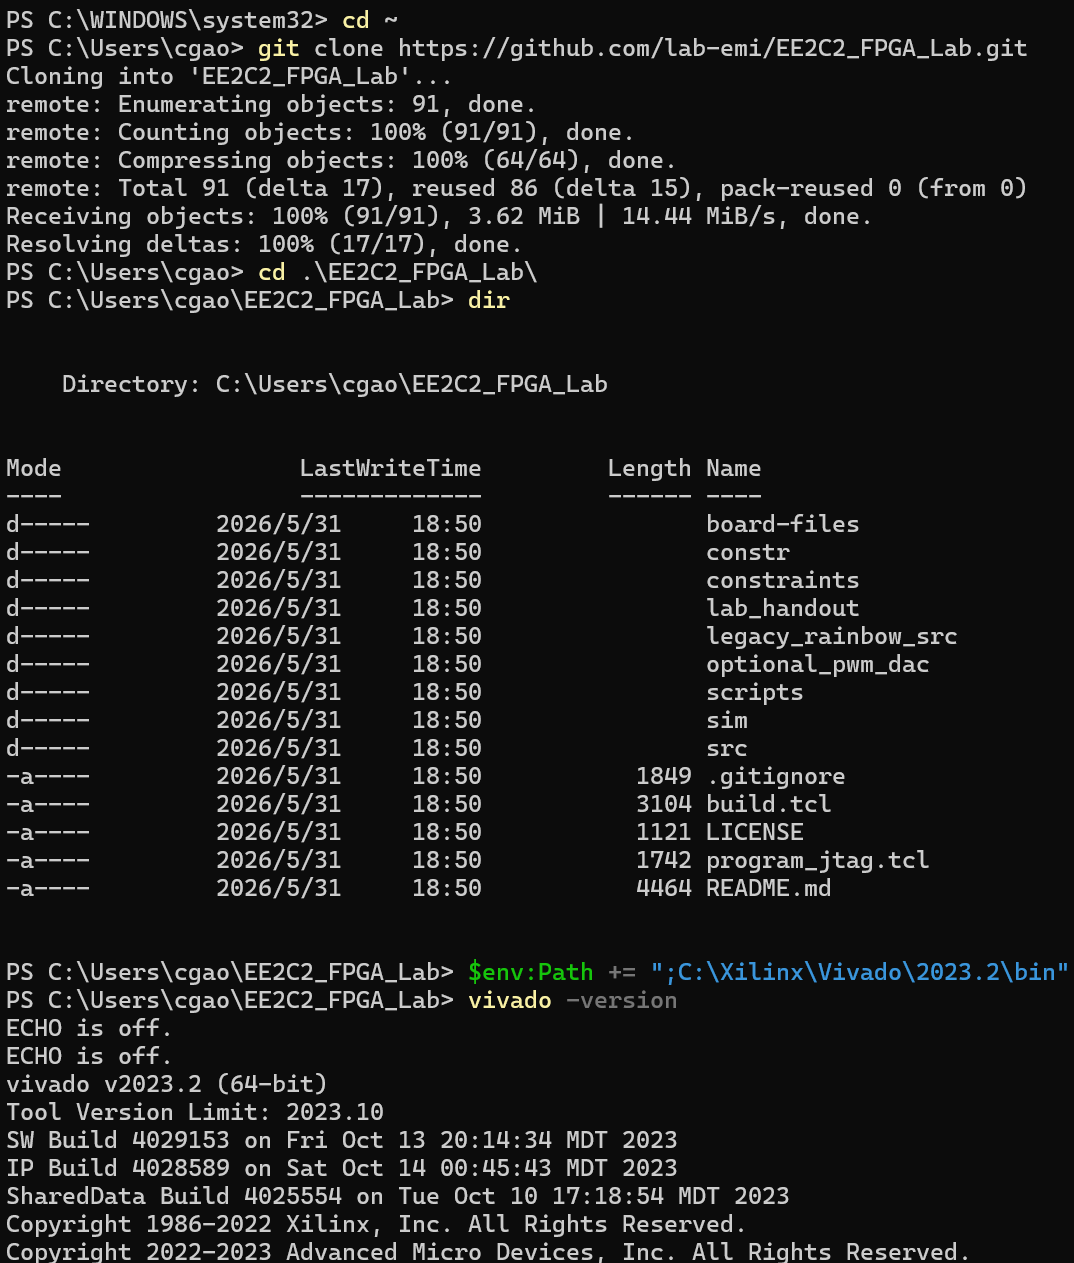
\includegraphics[width=0.7\linewidth]{Figures/screenshots/t0_02_powershell_setup.png}
  \caption{PowerShell ready in the cloned lab folder.}
\end{figure}

\paragraph{Step 0.2 --- Create the Vivado project.}

\pstag~ this builds the project without synthesis (fast):
\begin{lstlisting}[style=ps]
vivado -mode batch -source scripts\create_vivado_project.tcl
\end{lstlisting}
Watch for \texttt{INFO: Using AC701 implementation part: xc7a200tfbg676-2} and
\texttt{INFO: Created project: \ldots\textbackslash build\textbackslash EE2C2\_FPGA\_Lab.xpr}. This project
targets the AC701 board part \texttt{xilinx.com:ac701:part0:1.4}; it is the project you use for
simulation setup, synthesis, implementation, timing, and power reports.

\begin{notebox}
\texttt{create\_vivado\_project.tcl} deletes and recreates the \texttt{build\textbackslash} folder
every run. That is fine --- all sources live in \texttt{src\textbackslash}, \texttt{sim\textbackslash},
\texttt{constr\textbackslash}, never in \texttt{build\textbackslash}.
\end{notebox}

\begin{figure}[htbp]
  \centering
  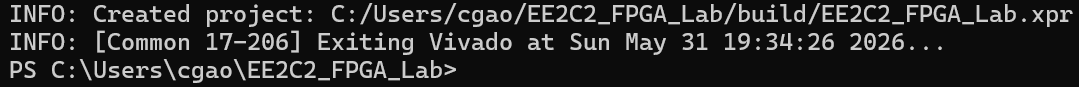
\includegraphics[width=0.85\linewidth]{Figures/screenshots/t0_03_create_project.png}
  \caption{Project created from the Tcl script.}
\end{figure}

\paragraph{Step 0.3 --- Open the project in the GUI.}

\pstag~
\begin{lstlisting}[style=ps]
vivado build\EE2C2_FPGA_Lab.xpr
\end{lstlisting}

\guitag~ \emph{(alternative)} Start menu \gto\ \nav{Vivado 2023.2} \gto\ \nav{Open Project} \gto\
select \texttt{build\textbackslash EE2C2\_FPGA\_Lab.xpr}.

Find the four areas you will use constantly: \nav{Flow Navigator} (left), \nav{Sources} (centre),
\nav{Tcl Console} (bottom), and \nav{Messages} (bottom). Try typing \texttt{version -short} in the
Tcl Console.

\begin{figure}[htbp]
  \centering
  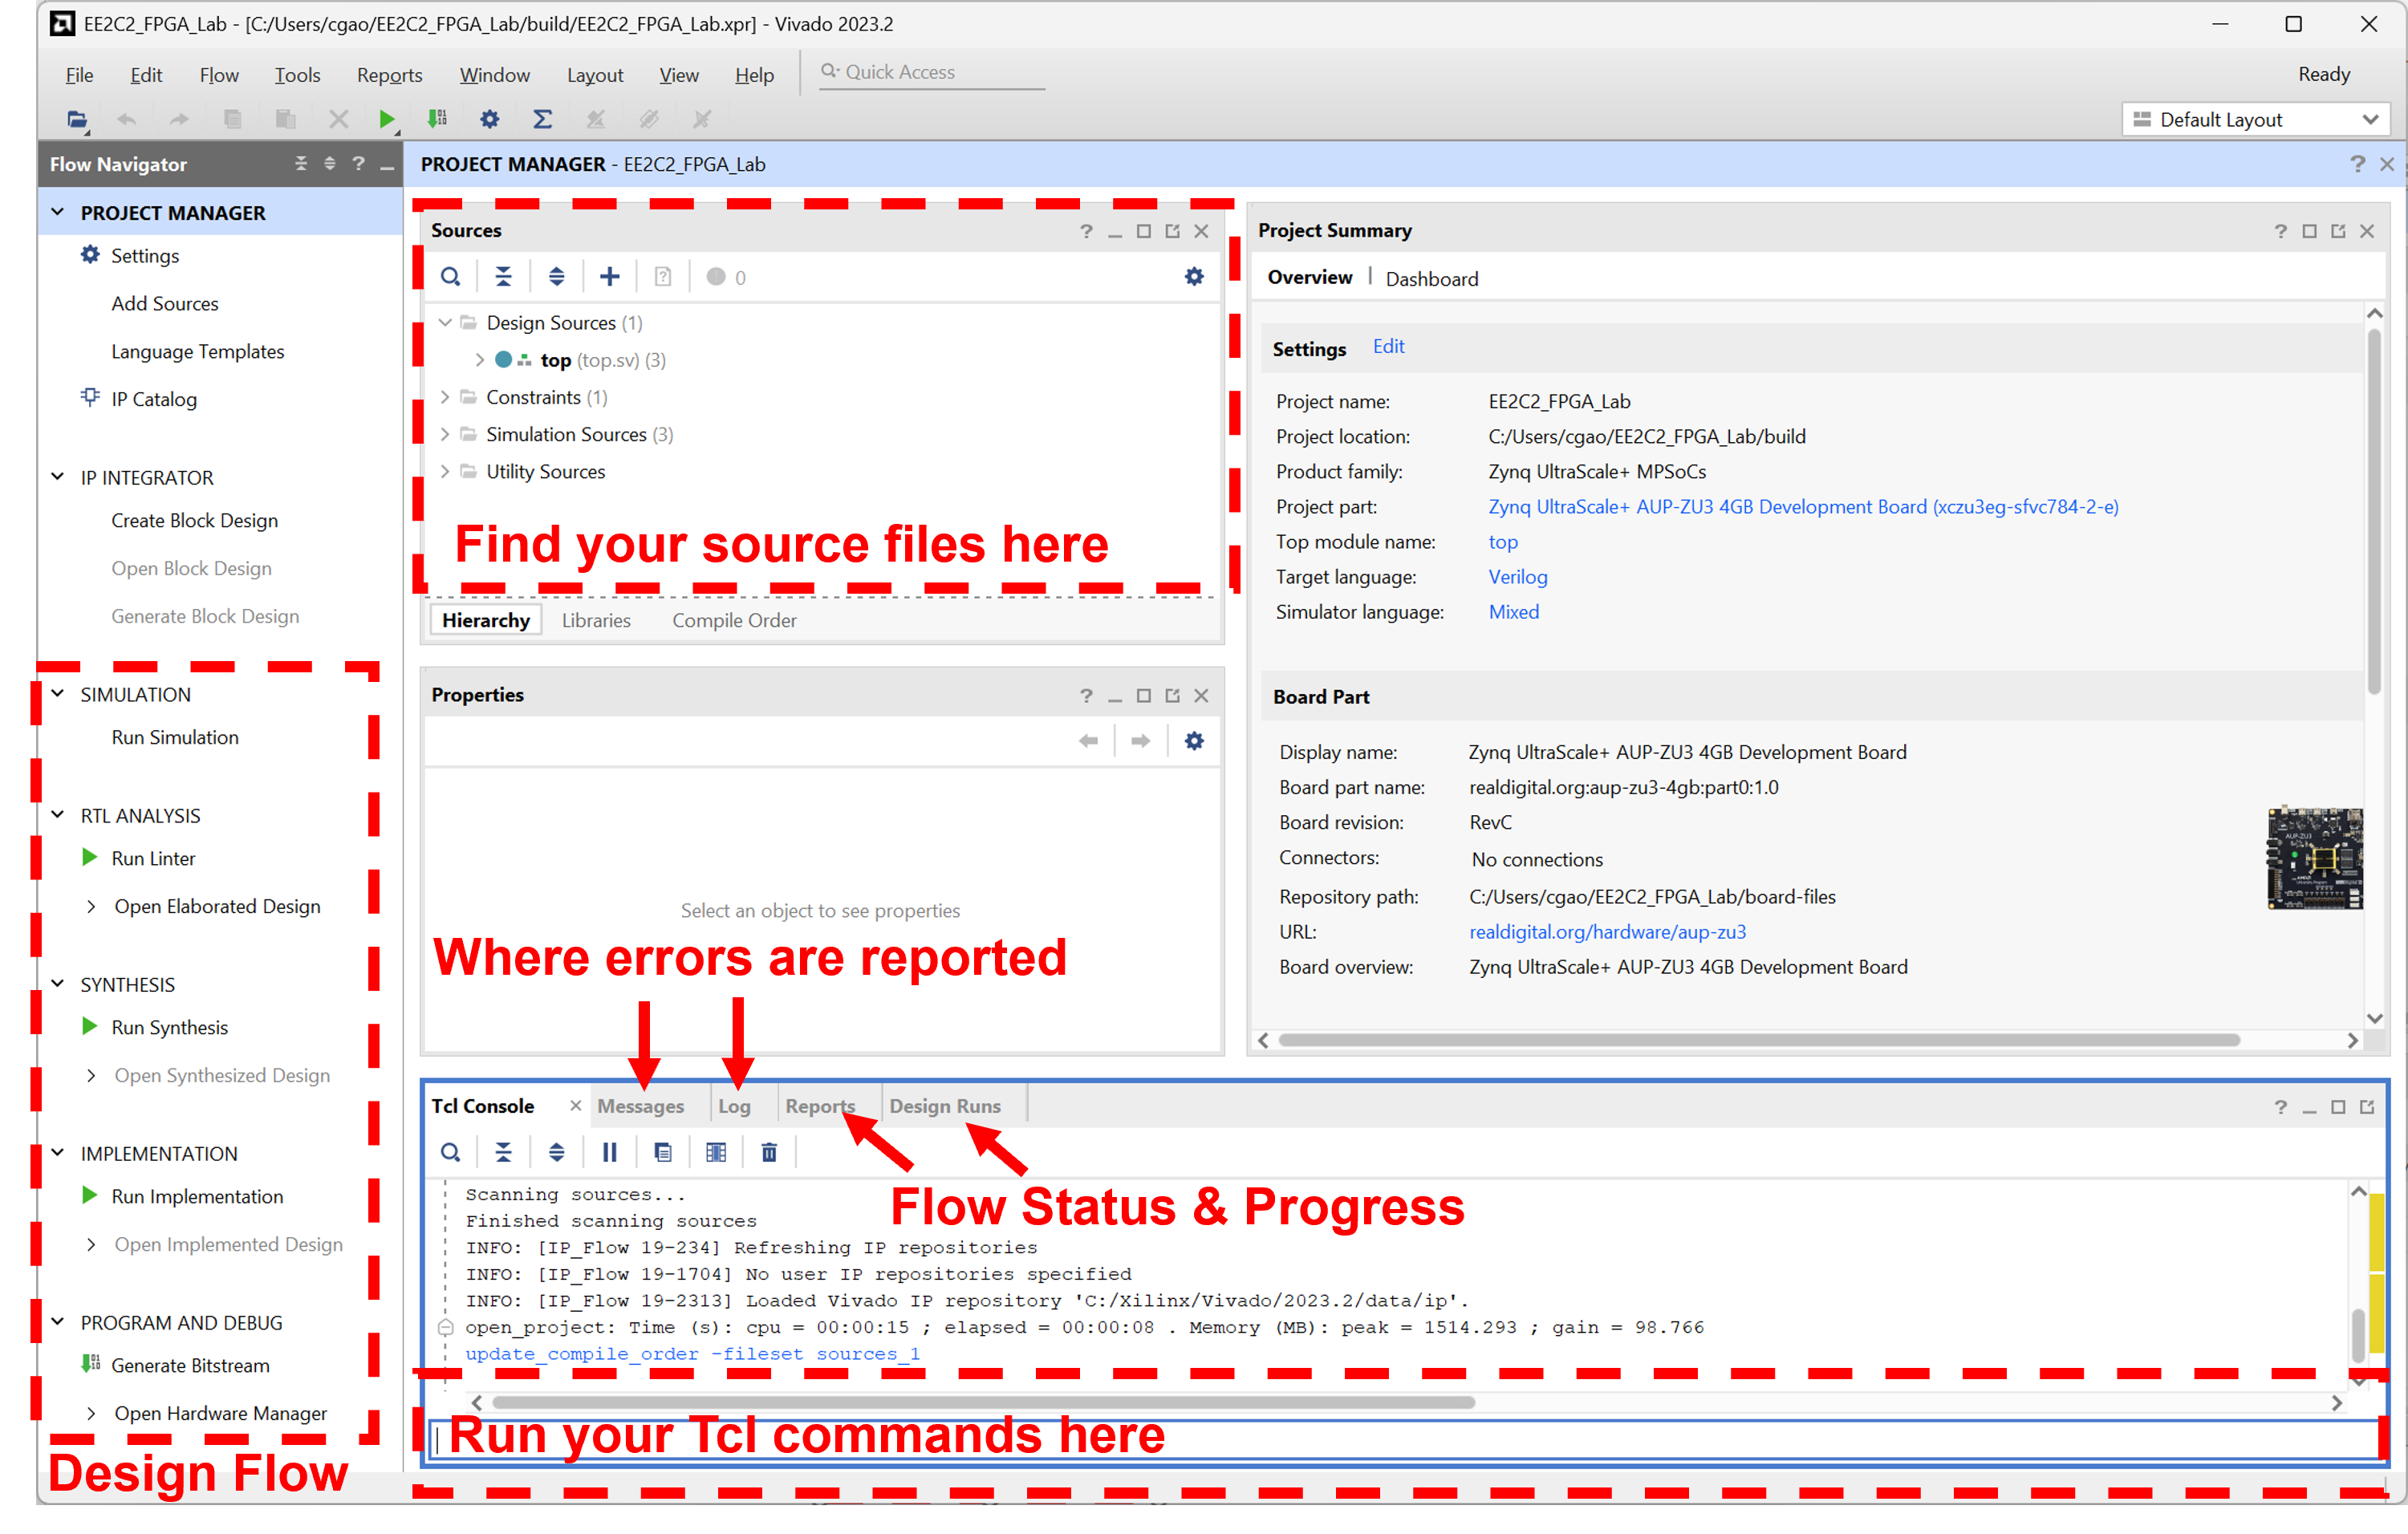
\includegraphics[width=0.95\linewidth]{Figures/screenshots/t0_04_vivado_main_window.png}
  \caption{The Vivado main window.}
\end{figure}

\paragraph{Step 0.4 --- Find the source files.}

\guitag~ In \nav{Sources}, expand \nav{Design Sources} (\texttt{top\_ac701},
\texttt{comb\_led\_logic}, \texttt{one\_hz\_tick}, \texttt{led\_fsm}), \nav{Constraints}
(\texttt{ac701\_lab.xdc}), and
\nav{Simulation Sources} (\texttt{tb\_comb\_led\_logic}, \texttt{tb\_led\_fsm}).

\tcltag~ \emph{(alternative)}
\begin{lstlisting}[style=tcl]
report_compile_order -fileset sources_1
get_files
\end{lstlisting}

\begin{figure}[htbp]
  \centering
  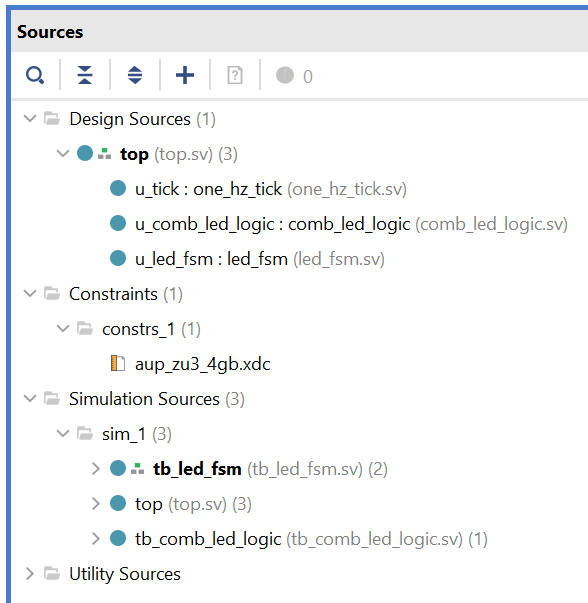
\includegraphics[width=0.5\linewidth]{Figures/screenshots/t0_05_sources_panel.png}
  \caption{The Sources panel, fully expanded.}
\end{figure}

\begin{questionbox}
\textbf{Checkpoint 0.} Confirm the project was created and record your Vivado version (2023.2).
\end{questionbox}

% ============================================================================
\newpage
\section{Topic 1 --- Combinational logic}

\subsection{Background}
\textbf{Combinational logic} produces outputs that depend \emph{only on the current inputs} ---
no memory. Examples: gates, multiplexers, decoders, comparators. In SystemVerilog you use
\texttt{assign} or an \texttt{always\_comb} block:
\begin{lstlisting}[style=sv]
assign y = (a & b) | (~a & c);
\end{lstlisting}
This does not ``execute'' like software --- it \emph{describes hardware that is always present}.
When \texttt{a}, \texttt{b}, or \texttt{c} changes, \texttt{y} settles after the gate delay.

\begin{notebox}
\textbf{Avoid latches.} Inside an \texttt{always\_comb}, assign every output on every path (the lab
code writes a default value first). An unassigned output infers an unwanted memory element (a latch).
\end{notebox}

\subsection{Lab 1: inspect and simulate the combinational logic}

\paragraph{Step 1.1 --- Open the source.}

\guitag~ \nav{Sources}\gto\nav{Design Sources}\gto double-click \texttt{comb\_led\_logic}.
Read the \texttt{always\_comb} block; note the default \texttt{led\_comb = 8'b0000\_0000;} that
prevents latches.
\begin{figure}[htbp]
  \centering
  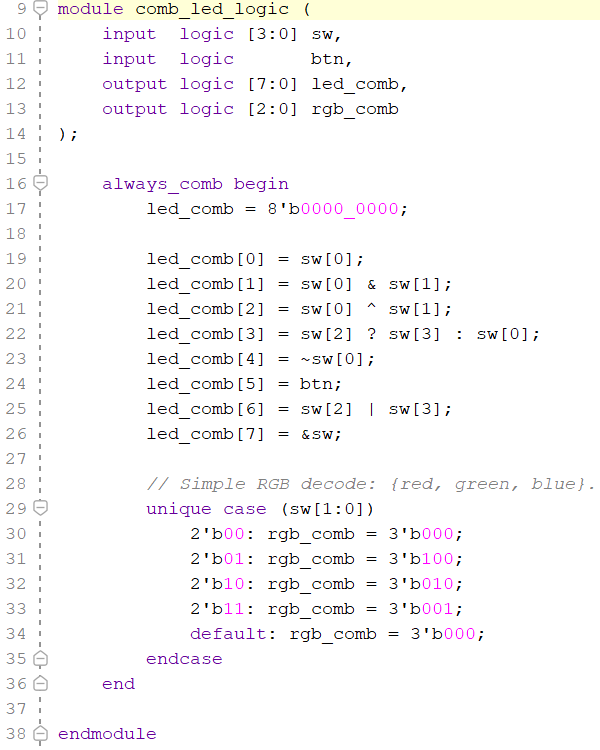
\includegraphics[width=0.5\linewidth]{Figures/screenshots/t1_01_comb_source.png}
  \caption{\texttt{comb\_led\_logic.sv} in the editor.}
\end{figure}

For example,\texttt{src/comb\_led\_logic.sv} contains some combinational logic examples that drive the single-colour LEDs in combinational mode:
\begin{lstlisting}[style=sv]
led_comb[1] = sw[0] & sw[1];          // ?
led_comb[2] = sw[0] ^ sw[1];          // ?
led_comb[3] = sw[2] ? sw[3] : sw[0];  // ?
led_comb[7] = &sw;                    // 4-input reduction AND
\end{lstlisting}

\begin{questionbox}
\textbf{Checkpoint 1a.} Which line is an \textbf{AND} gate, which is an \textbf{XOR} gate, and which is a \textbf{multiplexer}?
\end{questionbox}

\paragraph{Step 1.2 --- Make the combinational testbench the simulation top.}

\guitag~ \nav{Sources}\gto\nav{Simulation Sources}\gto\nav{sim\_1}\gto right-click
\texttt{tb\_comb\_led\_logic} \gto\ \nav{Set as Top}.\\
\tcltag~ \emph{(alternative)}
\begin{lstlisting}[style=tcl]
set_property top tb_comb_led_logic [get_filesets sim_1]
update_compile_order -fileset sim_1
\end{lstlisting}

\begin{figure}[htbp]
  \centering
  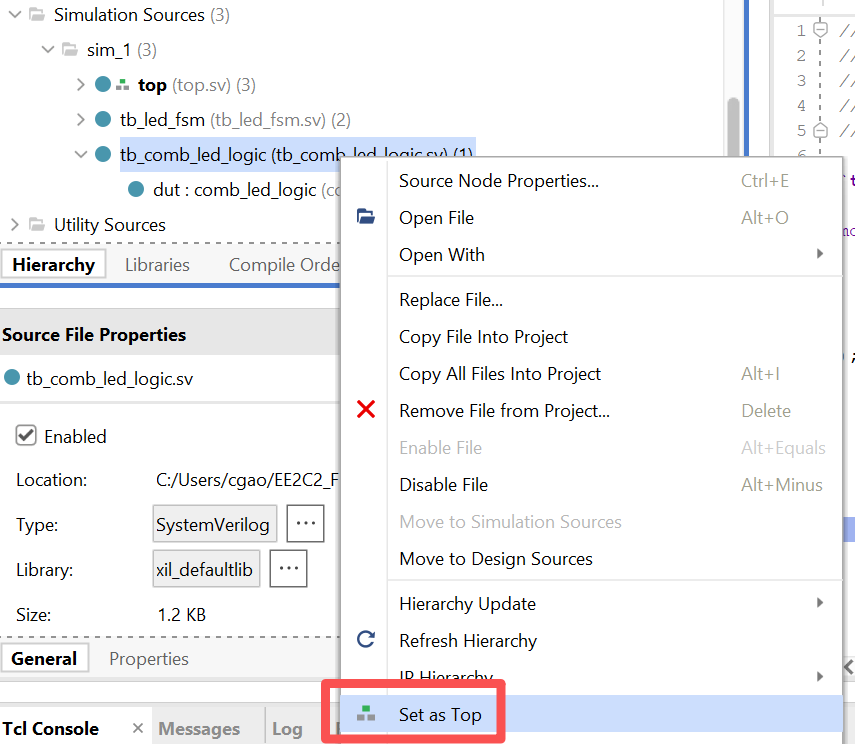
\includegraphics[width=0.85\linewidth]{Figures/screenshots/t1_02_set_as_top.png}
  \caption{Setting the simulation top.}
\end{figure}

\paragraph{Step 1.3 --- Run the behavioural simulation.}

\guitag~ \nav{Flow Navigator}\gto\nav{Run Simulation}\gto\nav{Run Behavioral Simulation}.\\
\begin{notebox}
\textbf{Close the previous simulation before launching another one.} If a waveform/simulator window is
still open, run \texttt{close\_sim} in the Tcl Console (or close the current simulation from the GUI)
before the next \texttt{launch\_simulation}. Otherwise Vivado may report
\texttt{ERROR: [Vivado 12-1501] Simulator for snapshot \ldots\ is already running}.
\end{notebox}
\tcltag~ \emph{(alternative)}
\begin{lstlisting}[style=tcl]
catch {close_sim} ;# harmless if no simulation is open
launch_simulation
run all
\end{lstlisting}

\pstag~ \emph{(alternative, no GUI)}
\begin{lstlisting}[style=ps]
vivado -mode batch -source scripts\run_simulation.tcl -tclargs tb_comb_led_logic
\end{lstlisting}
The Tcl console should print lines like \texttt{sw=1111 btn=0 led\_comb=\ldots} ending with
\texttt{tb\_comb\_led\_logic completed.}

\paragraph{Step 1.4 --- Read the waveform.}

\guitag~ Ensure \texttt{sw}, \texttt{btn}, \texttt{led\_comb}, \texttt{rgb\_comb} are visible; drag in
any missing signal and click \nav{Zoom Fit}. Observe that when \texttt{sw} changes, the outputs change
at the \emph{same} simulation time --- there is no clock here.

\begin{figure}[htbp]
  \centering
  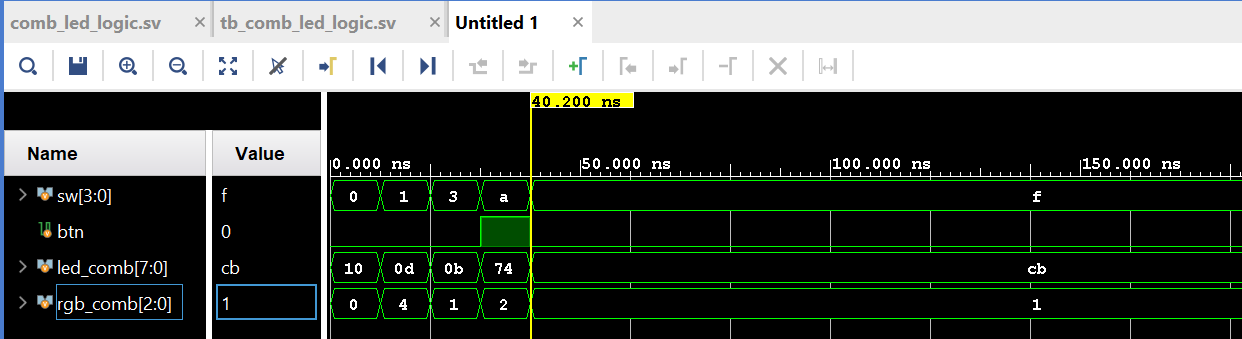
\includegraphics[width=1.0\linewidth]{Figures/screenshots/t1_03_comb_waveform.png}
  \caption{Behavioural-simulation waveform for the combinational logic.}
\end{figure}
\par\noindent\textit{Report evidence: capture the \texttt{tb\_comb\_led\_logic} waveform and mark one input change where the output changes at the same simulation time.}\par

\begin{questionbox}
\textbf{Checkpoint 1b.} Why can a \emph{testbench} change inputs with \texttt{\#10} delays, while
\emph{synthesizable} RTL must not use \texttt{\#10} delays?
\end{questionbox}

% ============================================================================
\newpage
\section{Topic 2 --- Sequential logic}

\subsection{Background}
\textbf{Sequential logic} has memory: outputs can depend on past inputs. State is stored in
\textbf{flip-flops} that update only on a \textbf{clock edge}.
\begin{itemize}[noitemsep]
  \item \texttt{always\_ff @(posedge clk)} describes flip-flops.
  \item \texttt{<=} (non-blocking) is used for clocked updates.
  \item A \textbf{counter} is the simplest example.
\end{itemize}
\begin{lstlisting}[style=sv]
always_ff @(posedge clk) begin
    if (rst) count <= '0;
    else     count <= count + 1'b1;
end
\end{lstlisting}
The lab module \texttt{src/one\_hz\_tick.sv} counts clock cycles and, on the wrap cycle, raises
\texttt{tick\_1s} for exactly one clock cycle. In the AC701 implementation, \texttt{top\_ac701.sv}
sets the counter limit for the 200\,MHz board clock.

\begin{notebox}
\textbf{A tick is a clock \emph{enable}, not a new clock.} \texttt{tick\_1s} is a normal signal that
is high for one cycle. The whole design still runs on the single 100\,MHz \texttt{clk}.
\end{notebox}

\subsection{Lab 2: inspect the counter and watch it tick}

\paragraph{Step 2.1 --- Open the source.}

\guitag~ \nav{Sources}\gto\nav{Design Sources}\gto double-click \texttt{one\_hz\_tick}. Find the
\texttt{always\_ff} block, the register \texttt{count\_value}, and the line that pulses \texttt{tick\_1s}.

\begin{figure}[htbp]
  \centering
  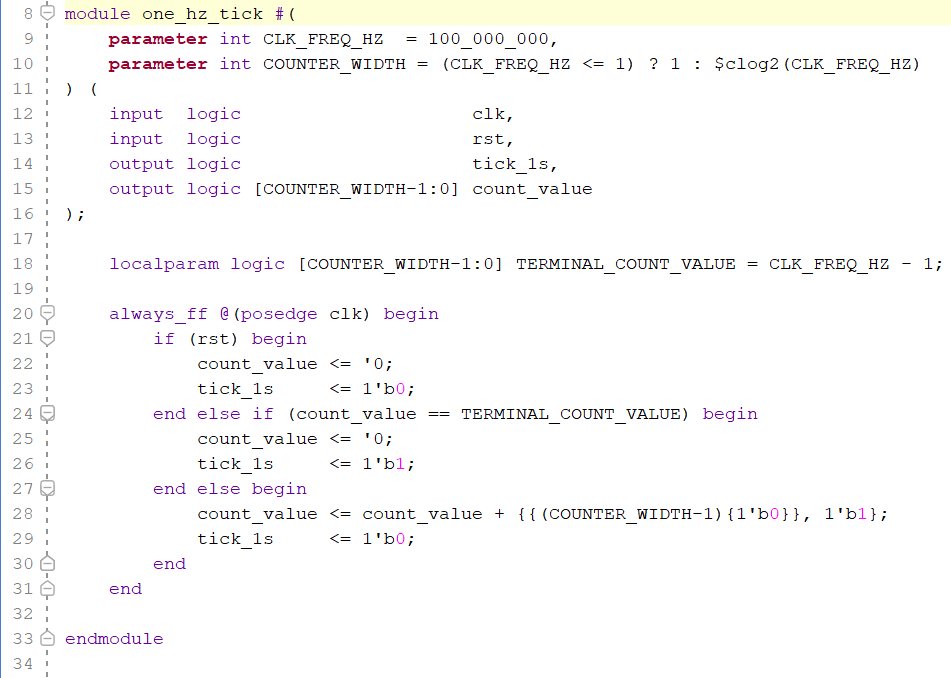
\includegraphics[width=0.76\linewidth]{Figures/screenshots/t2_01_tick_source.png}
  \caption{\texttt{one\_hz\_tick.sv} in the editor.}
\end{figure}

\paragraph{Step 2.2 --- Observe the counter and tick in simulation.}
The counter runs together with the FSM in \texttt{tb\_led\_fsm}, which uses a tiny
\texttt{SIM\_CLK\_FREQ\_HZ = 8} so a tick happens every 8 cycles. (Full run in Topic 3.)
\tcltag~
\begin{lstlisting}[style=tcl]
catch {close_sim} ;# close the Topic 1 simulation if it is still open
set_property top tb_led_fsm [get_filesets sim_1]
update_compile_order -fileset sim_1
launch_simulation
run all
\end{lstlisting}
Watch \texttt{count\_value} increment $0\to7$ and \texttt{tick\_1s} pulse for one cycle on each wrap.

\begin{figure}[htbp]
  \centering
  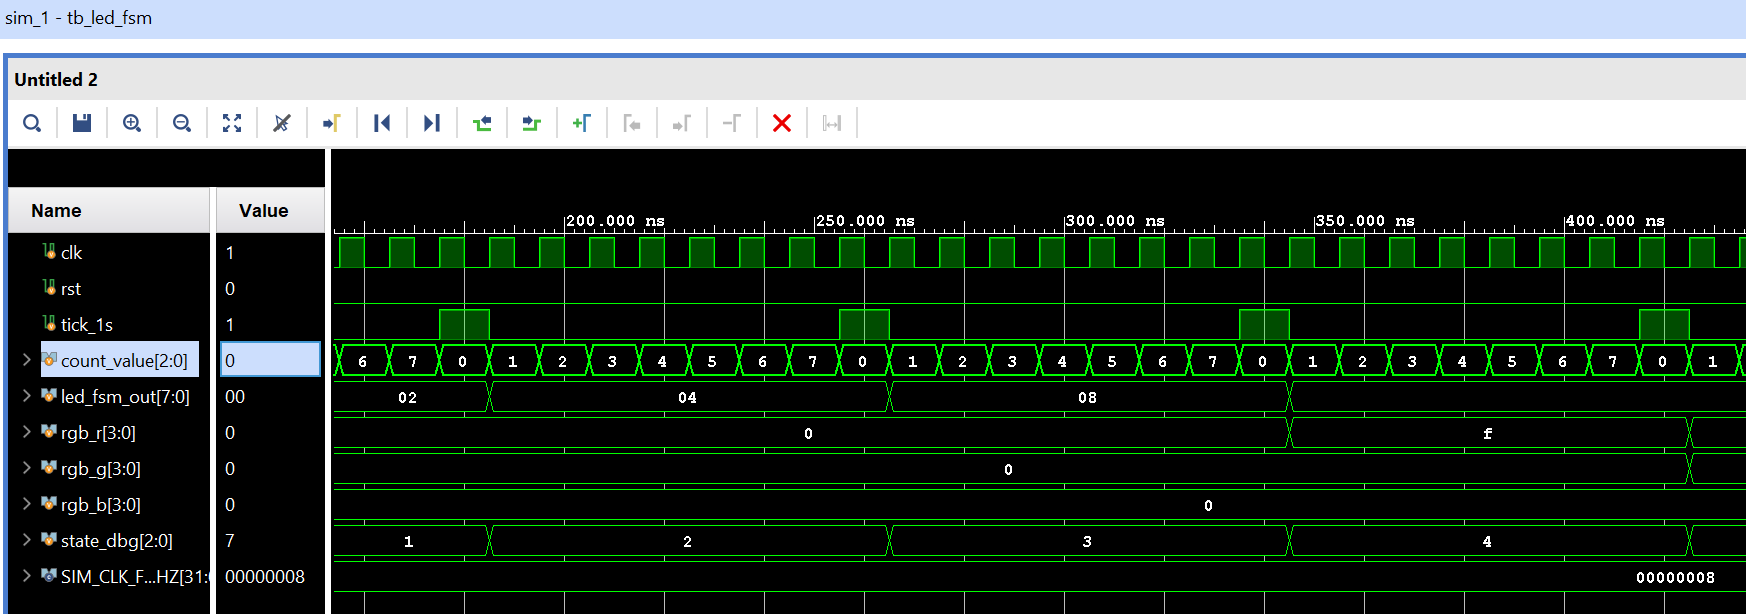
\includegraphics[width=1.0\linewidth]{Figures/screenshots/t2_02_counter_tick_waveform.png}
  \caption{Counter and tick in the FSM testbench.}
\end{figure}
\par\noindent\textit{Report evidence: capture a zoom of \texttt{count\_value} wrapping and the one-cycle \texttt{tick\_1s} pulse.}\par

\begin{questionbox}
\textbf{Checkpoint 2.} What hardware does \texttt{always\_ff @(posedge clk)} infer, and why is
\texttt{tick\_1s} a clock-enable pulse rather than a new clock?
\end{questionbox}

% ============================================================================
\newpage
\section{Topic 3 --- Finite state machines}

\subsection{Background}
A \textbf{finite state machine (FSM)} is sequential logic that moves through defined \textbf{states}.
It has three parts: a \textbf{state register} (flip-flops, \emph{sequential}), \textbf{next-state logic}
(\emph{combinational}), and \textbf{output decode logic} (\emph{combinational}). The lab FSM
(\texttt{src/led\_fsm.sv}) advances one step per tick:
\begin{lstlisting}[style=plain]
IDLE -> MONO_LED_0 -> MONO_LED_1 -> MONO_LED_2
     -> RGB_RED -> RGB_GREEN -> RGB_BLUE -> ALL_OFF -> (back to IDLE)
\end{lstlisting}
A transition happens \emph{only when} \texttt{tick\_1s} is high --- once per second on the board.

\begin{figure}[htbp]
  \centering
  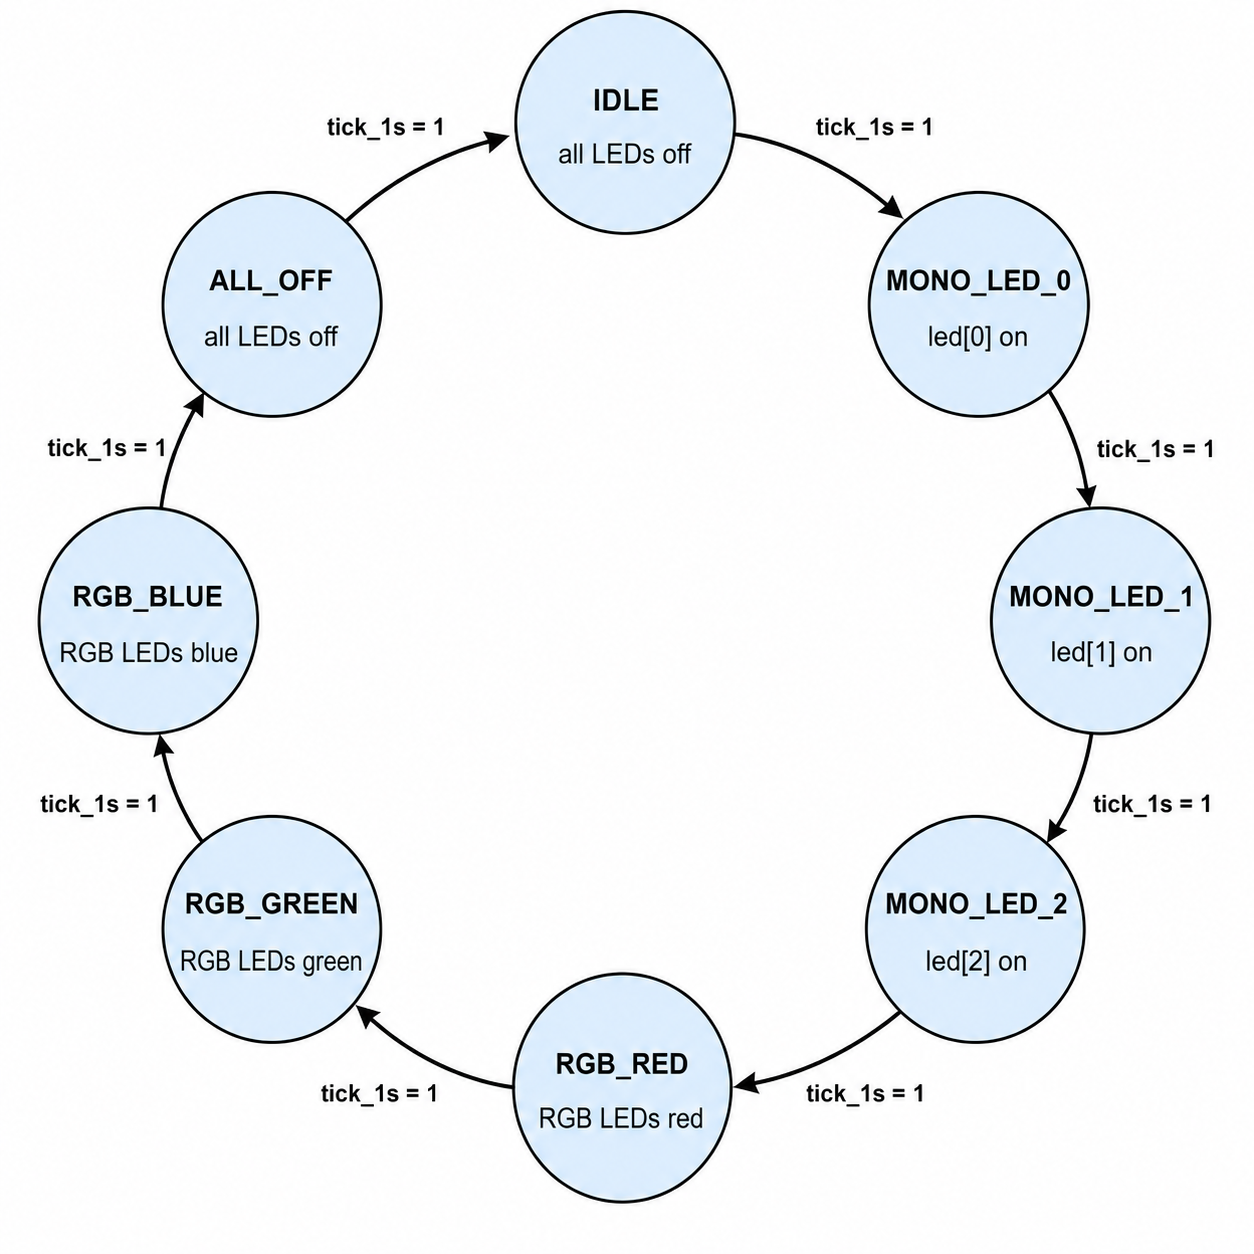
\includegraphics[width=0.85\linewidth]{Figures/screenshots/t3_01_fsm_state_diagram.png}
  \caption{FSM state diagram.}
\end{figure}

\subsection{Lab 3: inspect and simulate the FSM}

\paragraph{Step 3.1 --- Open and identify the three FSM parts.}

\guitag~ \nav{Sources}\gto\nav{Design Sources}\gto double-click \texttt{led\_fsm}. Locate (1) the
\texttt{typedef enum} state type, (2) the state register \texttt{always\_ff \ldots state <= next\_state;},
(3) the next-state \texttt{always\_comb} guarded by \texttt{if (tick\_1s)}, and (4) the output-decode
\texttt{always\_comb} that sets \texttt{led\_fsm}, \texttt{rgb\_r/g/b}.

\paragraph{Step 3.2 --- Run the FSM testbench.}

\guitag~ Make \texttt{tb\_led\_fsm} the sim top (right-click \gto\ \nav{Set as Top}), then
\nav{Flow Navigator}\gto\nav{Run Simulation}\gto\nav{Run Behavioral Simulation}.\\

\pstag~ \emph{(alternative)}
\begin{lstlisting}[style=ps]
vivado -mode batch -source scripts\run_simulation.tcl -tclargs tb_led_fsm
\end{lstlisting}
\tcltag~ \emph{(alternative)}
\begin{lstlisting}[style=tcl]
catch {close_sim} ;# close any previous simulation snapshot first
set_property top tb_led_fsm [get_filesets sim_1]
update_compile_order -fileset sim_1
launch_simulation
run all
\end{lstlisting}

\paragraph{Step 3.3 --- Read the FSM waveform.}

\guitag~ Add \texttt{clk}, \texttt{rst}, \texttt{tick\_1s}, \texttt{count\_value}, \texttt{state\_dbg},
\texttt{led\_fsm\_out}, \texttt{rgb\_r}, \texttt{rgb\_g}, \texttt{rgb\_b}; \nav{Zoom Fit}. Observe: reset
holds \texttt{IDLE}; after release, \texttt{tick\_1s} pulses every 8 clocks; \texttt{state\_dbg} advances
one state per tick; outputs follow the state. The console prints one line per tick, ending with
\texttt{tb\_led\_fsm completed.}

\begin{figure}[htbp]
  \centering
  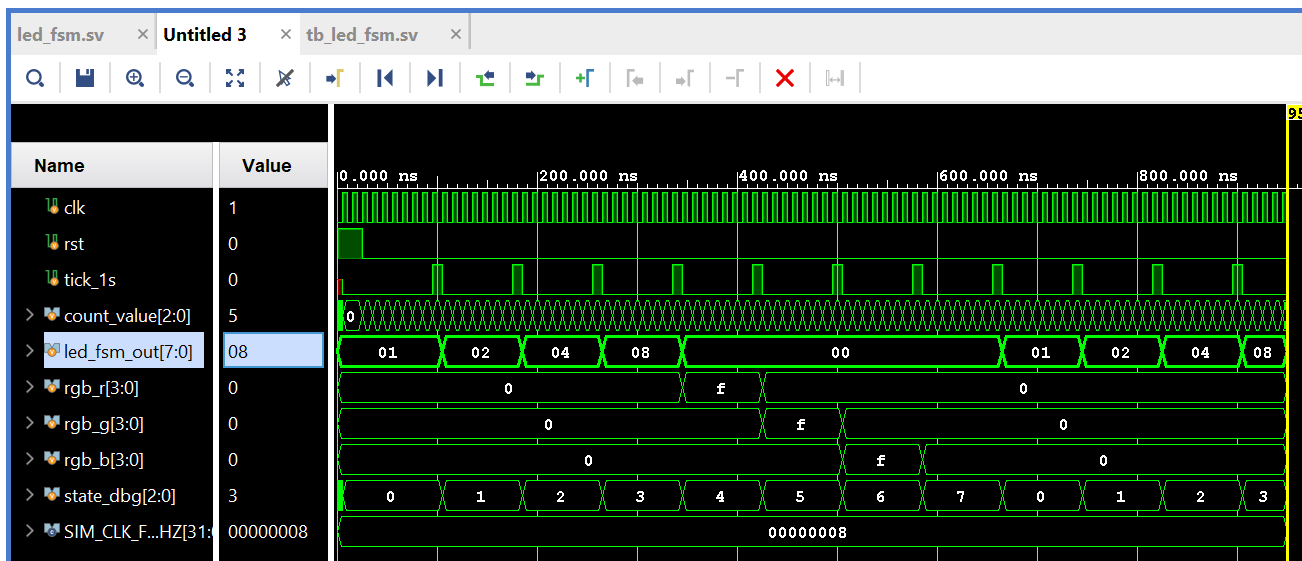
\includegraphics[width=1.0\linewidth]{Figures/screenshots/t3_03_fsm_waveform.png}
  \caption{The FSM testbench waveform.}
\end{figure}
\par\noindent\textit{Report evidence: capture the \texttt{tb\_led\_fsm} waveform and mark the reset region plus two consecutive \texttt{tick\_1s} pulses and their \texttt{state\_dbg} transitions.}\par

\begin{questionbox}
\textbf{Checkpoint 3.} Using the FSM waveform, choose two consecutive \texttt{tick\_1s} pulses after reset.
For each pulse, record the state just before the pulse, the state just after the pulse, and the LED/RGB
output after the transition. Then explain what this shows about the roles of the state register,
next-state logic, and output-decode logic.
\end{questionbox}

% ============================================================================
\newpage
\section{Topic 4 --- From RTL to bitstream: synthesis and implementation}

\subsection{Background}
The AC701 top \texttt{src/top\_ac701.sv} converts the differential clock with an \texttt{IBUFDS},
synchronises \texttt{rst\_btn}, instantiates the lab modules, and multiplexes between the FSM and
combinational LED outputs on \texttt{sw[3]}.
To reach a configured chip: \textbf{Synthesis} (RTL $\to$ LUT/FF netlist), \textbf{Implementation}
(place \& route onto this exact device), and \textbf{Bitstream generation} (\texttt{top\_ac701.bit}).

\subsection{Lab 4: build the design}
\begin{notebox}
\textbf{Do not run both methods at once.} \texttt{build.tcl} deletes and recreates
\texttt{build\textbackslash}. If the GUI has the project open, Windows blocks the delete.
\textbf{Close the GUI before running \texttt{build.tcl}}, or use the GUI buttons instead.
\end{notebox}

\paragraph{Option A --- one scripted build.}

\pstag~ (close the GUI first)
\begin{lstlisting}[style=ps]
vivado -mode batch -source build.tcl
\end{lstlisting}
Watch for \texttt{INFO: Bitstream generated at: \ldots\textbackslash impl\_1\textbackslash top\_ac701.bit}.

\paragraph{Option B --- click through the flow.}

\guitag~ \nav{Flow Navigator}\gto\nav{Run Synthesis} (\nav{OK}); when it finishes choose
\nav{Run Implementation} (\nav{OK}); then \nav{Generate Bitstream} (\nav{OK}).\\
\tcltag~ \emph{(equivalent)}
\begin{lstlisting}[style=tcl]
launch_runs synth_1 -jobs 4
wait_on_run synth_1
launch_runs impl_1 -to_step write_bitstream -jobs 4
wait_on_run impl_1
\end{lstlisting}


\paragraph{Step 4.1 --- Confirm it built and check for errors.}

\guitag~ Open the \nav{Design Runs} tab; \texttt{synth\_1} and \texttt{impl\_1} should show green check
marks. Open \nav{Messages} and confirm no red errors.

\begin{figure}[htbp]
  \centering
  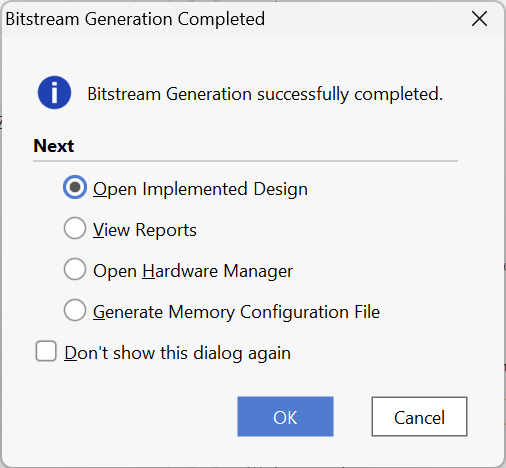
\includegraphics[width=0.3\linewidth]{Figures/screenshots/t4_02_runs_complete.png}
  \caption{Design Runs after a successful build. Open the implemented design to see reports.}
\end{figure}



\begin{questionbox}
\textbf{Checkpoint 4.} In one sentence,
what is the difference between synthesis and implementation?
\end{questionbox}

% ============================================================================
\newpage
\section{Topic 5 --- Hardware targets and AUP-ZU3 connection}

\subsection{Background}
The required implementation reports in this lab use the \textbf{AC701} project you built in Topic 4.
Your bench board is the \textbf{RealDigital AUP-ZU3-4GB}. Those are different FPGA families, so the
\texttt{top\_ac701.bit} file from Topic 4 must \textbf{not} be programmed onto the AUP-ZU3.

To keep the lab portable on university PCs, the AUP-ZU3 parts of the lab use \textbf{prebuilt AUP-ZU3
bitstreams}. Vivado only needs Hardware Manager to download those files over JTAG; it does not need to
synthesize, implement, or even create a project for the XCZU3EG device.

\subsection{Lab 5: prepare the AUP-ZU3 for prebuilt demos}

\paragraph{Step 5.1 --- Connect and power the AUP-ZU3.}
The board has \textbf{two USB-C ports}: \textbf{PROG UART} goes to the \textbf{PC} for JTAG/programming,
and \textbf{EXT PWR} goes to a USB-C \textbf{PD power adapter}. The PROG UART cable alone does not power
the board.

With the board \textbf{off}:
\begin{enumerate}
    \item set the \textbf{BOOT} switch next to the microSD slot to \textbf{JTAG}, not SD;
    \item connect the USB-A-to-USB-C data cable from the \textbf{PC} to \textbf{PROG UART};
    \item connect the USB-C PD adapter to \textbf{EXT PWR};
    \item power the board on and confirm the power LED turns on.
\end{enumerate}
\begin{figure}[htbp]
  \centering
  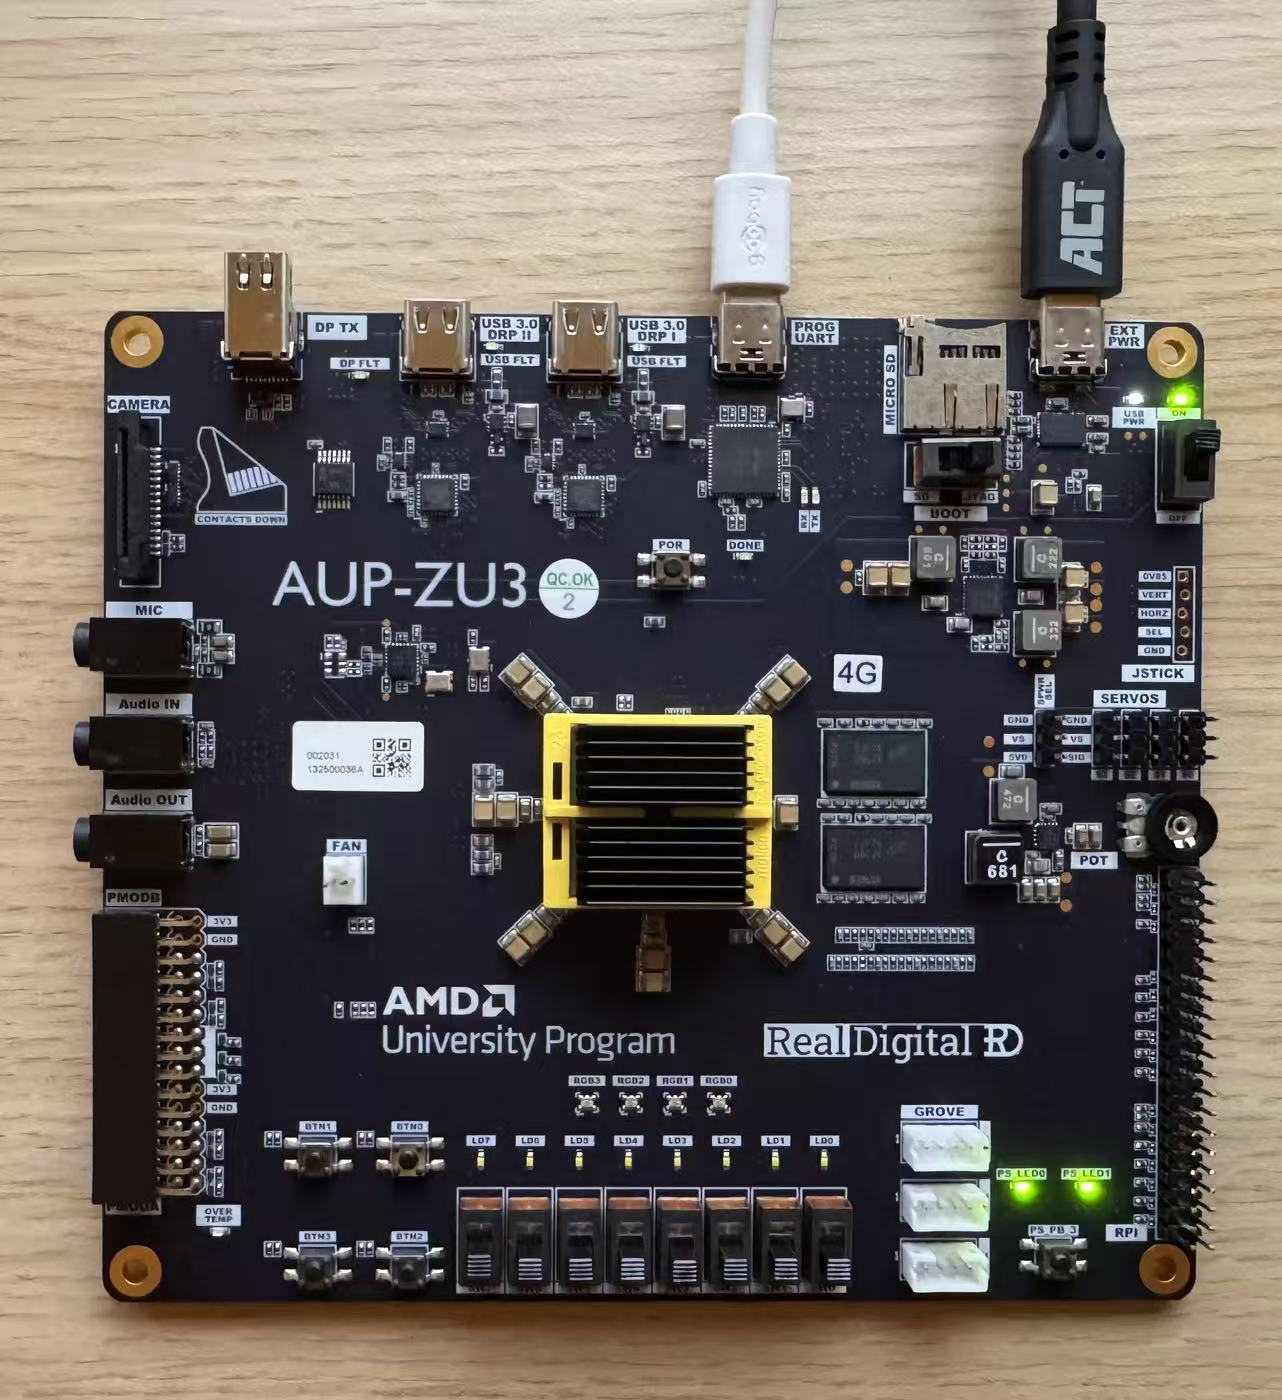
\includegraphics[width=0.4\linewidth]{Figures/screenshots/t5_01_board_connected.jpg}
  \caption{The powered AUP-ZU3 board with both USB-C cables attached.}
\end{figure}

\paragraph{Step 5.2 --- Check that Hardware Manager can see the board.}
\textbf{Preflight before any prebuilt demo:} \textbf{EXT PWR} is connected and the power LED is on;
\textbf{BOOT} is set to \textbf{USB-JTAG/JTAG} (power-cycle after changing it); \textbf{PROG UART} is
connected with a data cable; and no other Vivado, Vitis, Hardware Manager, or \texttt{hw\_server} session
is already using JTAG.

\guitag~ In Vivado, \nav{Open Hardware Manager}\gto\nav{Open Target}\gto\nav{Auto Connect}. The device
list should contain the FPGA device, usually named \texttt{xczu3\_0} or \texttt{xczu3eg}. You may also
see \texttt{arm\_dap\_1}; do not program that entry because it is the debug access port for the ARM
Processing System, not the FPGA fabric.

\tcltag~ The same check from a Tcl Console is:
\begin{lstlisting}[style=tcl]
open_hw_manager
connect_hw_server
open_hw_target
get_hw_devices
close_hw_target
close_hw_manager
\end{lstlisting}

\begin{figure}[htbp]
  \centering
  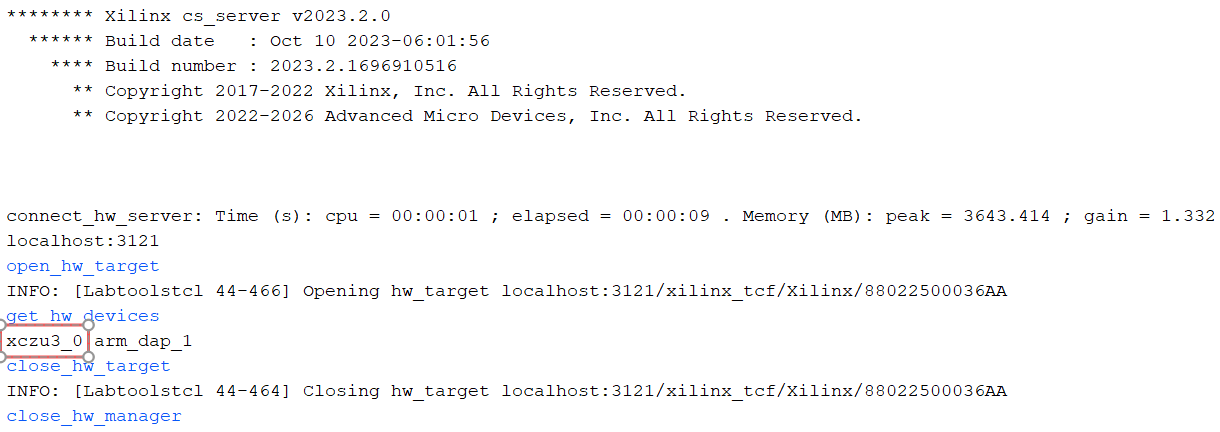
\includegraphics[width=1.0\linewidth]{Figures/screenshots/t5_05_hw_detected.png}
  \caption{The AUP-ZU3 detected in Hardware Manager.}
\end{figure}

\begin{notebox}
Use only one JTAG connection at a time. Close Hardware Manager before running a programming script, or
let the script open Hardware Manager itself. If a script says the target is busy, close other Vivado or
Vitis windows and retry.
\end{notebox}

\begin{questionbox}
\textbf{Checkpoint 5.} Why do Topics 4, 6, and 7 use the AC701 project, while the AUP-ZU3 board demos
use prebuilt bitstreams? In one sentence, also state why \texttt{top\_ac701.bit} must not be programmed
onto the AUP-ZU3.
\end{questionbox}

\paragraph{Troubleshooting}
If \nav{Auto Connect} finds nothing, or a prebuilt demo script reports that no FPGA device was found:
\begin{itemize}[noitemsep]
  \item \textbf{Power} --- is \textbf{EXT PWR} plugged in and the power LED on? \texttt{PROG UART} alone does not power the board.
  \item \textbf{Boot mode} --- is the \textbf{BOOT} switch on \textbf{JTAG} (not SD)? Power-cycle after changing it.
  \item \textbf{JTAG busy} --- close any other Vivado/Vitis or running script holding the target.
  \item \textbf{Wrong target} --- program the \texttt{xczu3}/\texttt{xczu3eg} FPGA device, not \texttt{arm\_dap}.
\end{itemize}

% ============================================================================
\newpage
\section{Topic 6 --- Static timing analysis}

\subsection{Background}
In the AC701 implementation the board clock is 200\,MHz, so the clock period is 5\,ns. Every signal launched
by one flip-flop on a clock edge must arrive at the capturing flip-flop, and settle,
\emph{before} the next edge. Static timing analysis (STA) checks this for \emph{all}
register-to-register paths without simulating any input vectors.

\paragraph{Setup constraint (data must not arrive too late).}
\[
  T_{\mathrm{clk}} \;\ge\; T_{\mathrm{clk\text{-}to\text{-}q}}
  + T_{\mathrm{comb}}^{\max} + T_{\mathrm{setup}} + \mathrm{margin}.
\]
The longest combinational path sets the maximum usable clock frequency: if the data
arrives after the setup window opens, the captured value is undefined.

\paragraph{Hold constraint (data must not arrive too early).}
\[
  T_{\mathrm{clk\text{-}to\text{-}q}} + T_{\mathrm{comb}}^{\min}
  \;\ge\; T_{\mathrm{hold}} + T_{\mathrm{skew}}.
\]
The \emph{shortest} path must be long enough that the new value does not race
through and overwrite the data before the capturing flip-flop has latched the
\emph{previous} value. Note this is independent of clock frequency. A hold
violation cannot be fixed by slowing the clock.

\paragraph{Slack.}
\[
  \mathrm{slack} = T_{\mathrm{required}} - T_{\mathrm{arrival}}.
\]
Positive slack means the path meets timing with margin to spare; negative slack
means it fails. Vivado reports the following:
\begin{itemize}[noitemsep]
  \item \textbf{WNS} --- Worst Negative Slack: the slack of the single tightest
        setup path. $\mathrm{WNS} \ge 0$ means \emph{every} setup path is met.
  \item \textbf{TNS} --- Total Negative Slack: the sum of all negative setup
        slacks. $\mathrm{TNS} = 0$ confirms there are no setup violations.
  \item \textbf{WHS / THS} --- Worst / Total Hold Slack, the hold-side
        equivalents of WNS / TNS.
  \item \textbf{Critical path} --- the path with the smallest slack, i.e.\ the
        one closest to failing (and the first to fix if timing is not met).
\end{itemize}
In this small design the critical path usually lies inside the one-second
counter, where the wide comparator and adder form the longest combinational
chain.

\subsection{Lab 6: read the timing report and find the critical path}

\paragraph{Step 6.1 --- Open the implemented design.}

\guitag~ \nav{Flow Navigator}\gto\nav{Open Implemented Design}.\quad

\tcltag~ \texttt{open\_run impl\_1}

\paragraph{Step 6.2 --- Open the timing summary.}

\guitag~ \nav{Reports}\gto\nav{Timing}\gto\nav{Report Timing Summary} (\nav{OK}).\\
\tcltag~ \texttt{report\_timing\_summary} \quad

\paragraph{Step 6.3 --- Inspect the worst (critical) path.}

\guitag~ In the \nav{Timing} tab expand \nav{Setup}\gto your clock and click the first (worst) path.
The \nav{Path Properties} show Source (From), Destination (to), Source Clock, Destination Clock, Total Delay, Logic Delay and Net Delay. Record them.

\paragraph{Step 6.4 --- See the path as hardware.}

\guitag~ Right-click the selected path \gto\ \nav{Schematic}. Identify the launch flip-flop, the
combinational logic (LUTs / carry chain), and the capture flip-flop.
\par\noindent\textit{Report evidence: capture the timing summary and/or the critical-path schematic with the launch flip-flop, logic, and capture flip-flop labelled.}\par

\begin{questionbox}
\textbf{Checkpoint 6.} Record WNS and TNS; state whether timing is met and how you know; record the
critical path start/endpoint; and describe the path in one sentence with a screenshot of the schematic attached.
\end{questionbox}

% ============================================================================
\newpage
\section{Topic 7 --- Power analysis}

\subsection{Background}
Vivado's power report \emph{estimates} on-chip power and splits it into two parts:
\textbf{static} power (transistor leakage, present whenever the device is powered)
and \textbf{dynamic} power (drawn only when nodes switch). Vivado further breaks the
dynamic part into \textbf{clock}, \textbf{logic/signal}, and \textbf{I/O} power.

Dynamic switching power follows
\[
  P_{\mathrm{dyn}} \;\approx\; \alpha\, C\, V_{\mathrm{DD}}^{2}\, f,
\]
where $\alpha$ is the switching (toggle) activity, $C$ the switched capacitance,
$V_{\mathrm{DD}}$ the supply voltage, and $f$ the clock frequency. The activity
$\alpha$ is the key unknown: unless you supply real switching data (e.g.\ a SAIF
file from simulation), Vivado performs a \emph{vectorless} estimate using assumed
default toggle rates, and flags this with a low \nav{Confidence level}. The
$V_{\mathrm{DD}}^{2}$ term is why supply voltage dominates the energy budget, and
the linear $f$ term is why the clock and clock-driven logic are often the largest
dynamic contributors.

\subsection{Lab 7: read the power report}

\paragraph{Step 7.1 --- Open the power report.}

\guitag~ \nav{Reports}\gto\nav{Report Power} (\nav{OK}).\\
\tcltag~ \texttt{report\_power}\\

\paragraph{Step 7.2 --- Record the numbers.}
From the \nav{Summary}, record the total on-chip power, the static and dynamic
totals, and the clock / logic-signal / I/O components; note which is largest.
Also record the reported \nav{Confidence level}, as it tells you how much to trust
the estimate.
\par\noindent\textit{Report evidence: capture the Power Summary panel with total power, static/dynamic split, and the largest category visible.}\par

\begin{questionbox}
\textbf{Checkpoint 7.}
\begin{enumerate}[noitemsep,nosep]
  \item Which power category is largest, and does the $\alpha C V_{\mathrm{DD}}^{2} f$
        relation explain why?
  \item What assumptions drive the estimate, and what would you provide to improve
        its confidence level?
  \item Does this report include the power consumed by the physical LEDs on the
        board?
\end{enumerate}
\end{questionbox}

% ============================================================================
\newpage
\section{Topic 8 --- PWM DAC: the digital/analog boundary}

\subsection{Background}
\textbf{Pulse-Width Modulation (PWM)} encodes an analog level as the fraction of time a digital signal
is high (the \textbf{duty cycle}). A free-running counter compares against \texttt{duty}:
\texttt{pwm\_out = (count < duty)}, so \texttt{pwm\_out} is high for \texttt{duty} of every $2^N$ cycles.
\begin{itemize}[noitemsep]
  \item With $N=8$, one period is $2^8=256$ cycles, so the PWM frequency is
        $100\,\mathrm{MHz}/256 = 390.625\,\mathrm{kHz}$.
  \item The selector maps \texttt{sw[3:0]} to \texttt{duty = \{sw, 4'b0000\}}: \texttt{0000}$\to$0\%,
        \texttt{1111}$\to 240/256 \approx 93.75\%$ (this simple version never reaches true 100\%).
\end{itemize}
An LED driven by PWM looks dimmer/brighter because the eye averages the fast on/off. In this lab we keep
the hardware simple and drive only the on-board LED. The same PWM idea can be filtered in other designs,
but there is no PMOD output in this version.

\begin{figure}[htbp]
  \centering
  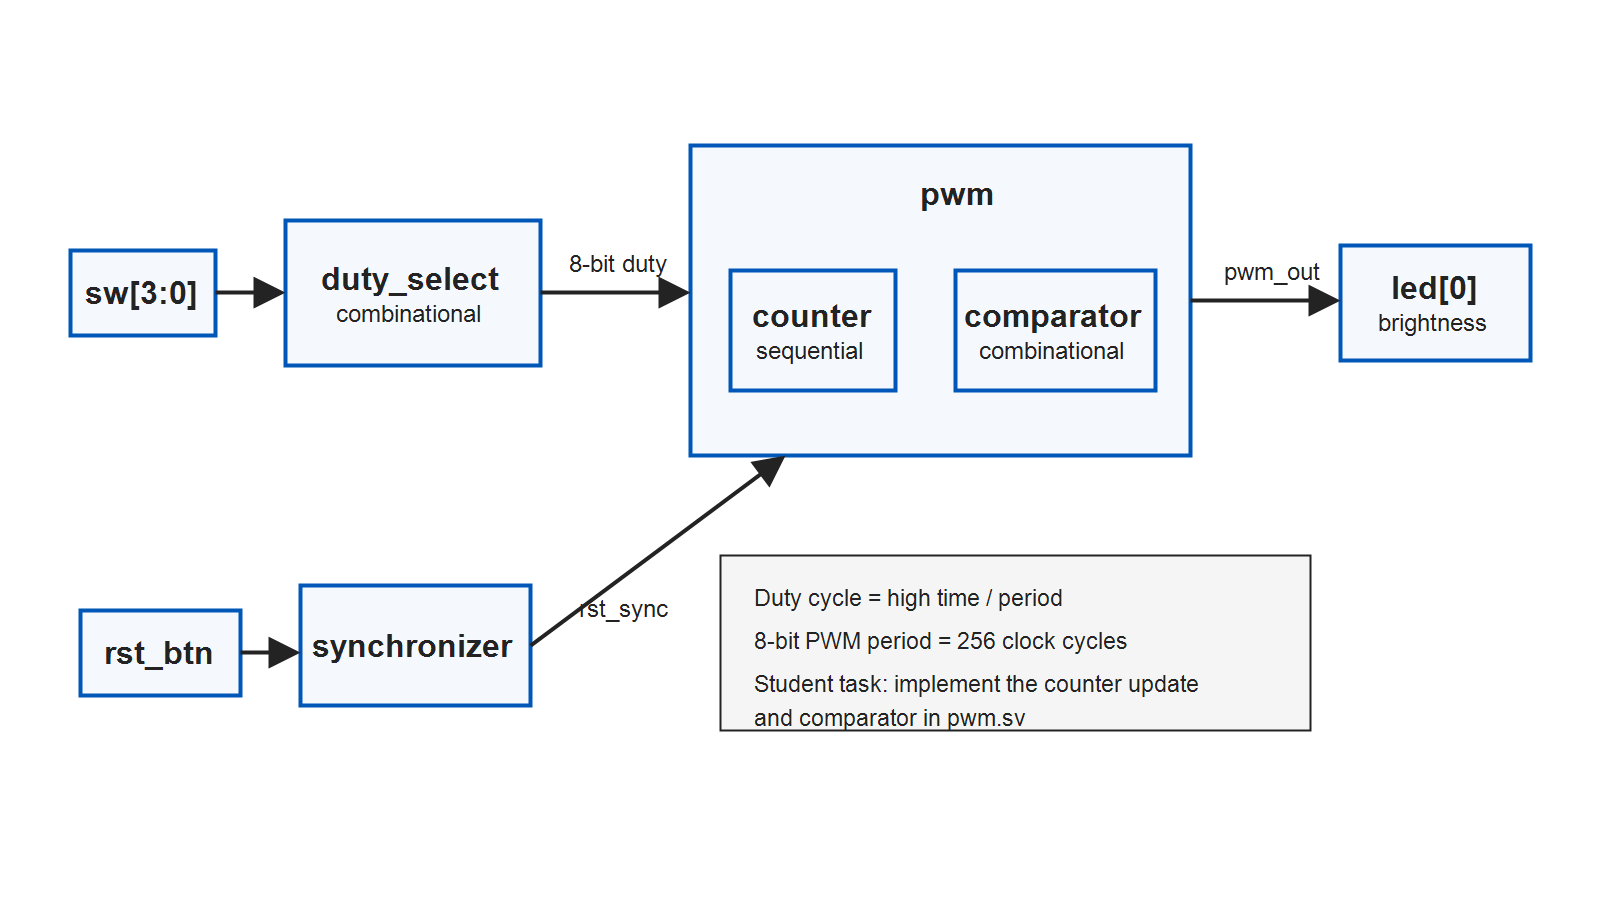
\includegraphics[width=1.0\linewidth]{Figures/screenshots/t8_01_pwm_datapath.png}
  \caption{The PWM data path.}
\end{figure}



\subsection{Lab 8: complete, simulate, and optionally observe the PWM LED dimmer}

\paragraph{Step 8.1 --- Complete the PWM mechanism.}
Skim the PWM source files:
\begin{itemize}[noitemsep]
  \item \texttt{pwm\_dac/src/duty\_select.sv}: combinational duty selection.
  \item \texttt{pwm\_dac/src/pwm.sv}: sequential counter plus combinational comparator.
  \item \texttt{pwm\_dac/src/synchronizer.sv}: reset-button synchronizer.
  \item \texttt{pwm\_dac/src/top\_pwm\_dac.sv}: top-level wiring.
\end{itemize}
Then open \texttt{pwm\_dac/src/pwm.sv} and fill in the two TODO lines:
\begin{enumerate}[noitemsep]
  \item update the N-bit counter once per clock when reset is not asserted;
  \item drive \texttt{pwm\_out} high when \texttt{count < duty}.
\end{enumerate}

\paragraph{Step 8.2 --- Simulate the PWM generator.}
\texttt{pwm\_dac/sim/tb\_pwm.sv} drives several duty values and checks \texttt{pwm\_out} is high for exactly
\texttt{duty} cycles per 256-cycle period. Run it only after completing \texttt{pwm.sv}.

\pstag~
Run the scripted simulation:
\begin{lstlisting}[style=ps]
vivado -mode batch -source pwm_dac\scripts\run_pwm_simulation.tcl
\end{lstlisting}
If the TODO lines are correct, the console and \texttt{pwm\_dac/build\_pwm\_dac/xsim\_pwm/xsim.log}
will include a clear pass line:
\begin{lstlisting}[style=plain]
PWM_STUDENT_TEST_PASS: all 7 duty-cycle checks passed.
\end{lstlisting}
If it fails, read the first \texttt{[FAIL]} or compile error, fix \texttt{pwm\_dac/src/pwm.sv}, and rerun.

\textbf{Before answering the Topic 8 worksheet, show your responsible TA the
\texttt{PWM\_STUDENT\_TEST\_PASS} line.} This is the required check for your own PWM implementation.
\par\noindent\textit{Report evidence: capture the console or \texttt{xsim.log} line showing
\texttt{PWM\_STUDENT\_TEST\_PASS}.}\par

\paragraph{Step 8.3 --- Optional prebuilt AUP-ZU3 brightness demo.}
The university PC may not be able to implement an XCZU3EG design, so the board demonstration uses a
prebuilt AUP-ZU3 bitstream from \texttt{prebuilt\_bitstreams/}. This demo shows the expected LED
brightness behavior; it is not proof that your TODO lines are correct. Your required proof is the
passing testbench from Step 8.2.

\pstag~ After the AUP-ZU3 connection preflight in Topic 5, program the prebuilt demo:
\begin{lstlisting}[style=ps]
vivado -mode batch -source pwm_dac\scripts\program_prebuilt_pwm_jtag.tcl
\end{lstlisting}
Set \texttt{sw[3:0]} low (e.g.\ \texttt{0001}) --- \texttt{led[0]} is dim; raise toward \texttt{1111} ---
brighter. \texttt{led[4:1]} mirrors your switch code.

\begin{questionbox}
\textbf{Checkpoint 8.}
\begin{enumerate}[noitemsep]
    \item For a 100\,MHz clock and 8-bit counter, what is the PWM frequency (show the arithmetic)?
    \item Why does changing duty change LED brightness?
    \item Which TODO line describes sequential logic, and which describes combinational logic?
    \item Why does \texttt{sw[3:0]=1111} not produce a true 100\% duty cycle in this selector?
\end{enumerate}
\end{questionbox}

% ============================================================================
\newpage
\section{Topic 9 --- Optional rainbow RTL demo}

\subsection{Just for fun}
If your group finishes early, you can program a prebuilt rainbow demo for the AUP-ZU3. It drives the
four RGB LEDs through a slowly changing hue generator. The switches still mirror onto the single-colour
LEDs, and the pushbuttons change the rainbow speed, direction, and phase spacing.

\paragraph{Step 9.1 --- Program the prebuilt rainbow demo.}
Keep the same AUP-ZU3 connection and JTAG preflight from Topic 5, then program the prebuilt rainbow
bitstream:
\begin{lstlisting}[style=ps]
vivado -mode batch -source rainbow\scripts\program_prebuilt_rainbow_jtag.tcl
\end{lstlisting}

\paragraph{Step 9.2 --- Play with the controls.}
\begin{itemize}[noitemsep]
  \item \texttt{sw[7:0]} mirror directly onto \texttt{led[7:0]}.
  \item Button 0 makes the colour cycle faster.
  \item Button 1 makes the colour cycle slower.
  \item Button 2 reverses the colour direction.
  \item Button 3 changes the phase spacing between RGB LEDs.
\end{itemize}

\begin{notebox}
Topic 9 is optional and has no report worksheet questions. It is a small reward lap after the required
PWM testbench pass is checked by your TA.
\end{notebox}

\subsection*{Lab completion checklist}
Your group passes the full lab flow if you ran at least one behavioural simulation, completed the AC701
implementation, recorded timing and power report values, identified a critical path, completed the PWM
TODOs, showed the \texttt{PWM\_STUDENT\_TEST\_PASS} line to your responsible TA, and answered the
checkpoint questions with reasonable understanding. The prebuilt AUP-ZU3 PWM and rainbow bitstreams are
for demonstration only.

\begin{notebox}
\textbf{Board return is required.} Your group can only pass the lab after returning the FPGA board box
to the responsible TA.
\end{notebox}

% ============================================================================
\appendix
\section{Command quick reference}
Run PowerShell commands from the \textbf{repository root} (the \texttt{EE2C2\_FPGA\_Lab} folder you cloned)
after adding Vivado to \texttt{\$env:Path} in Topic 0.

\begin{center}
\begin{tabular}{@{}p{4.6cm}p{9cm}@{}}
\toprule
\textbf{Task} & \textbf{Command} \\ \midrule
Clone the lab & \texttt{git clone https://github.com/lab-emi/EE2C2\_FPGA\_Lab.git} \\
Create project (no build) & \texttt{vivado -mode batch -source scripts\textbackslash create\_vivado\_project.tcl} \\
Open project in GUI & \texttt{vivado build\textbackslash EE2C2\_FPGA\_Lab.xpr} \\
Combinational sim & \texttt{vivado -mode batch -source scripts\textbackslash run\_simulation.tcl -tclargs tb\_comb\_led\_logic} \\
FSM sim & \texttt{vivado -mode batch -source scripts\textbackslash run\_simulation.tcl -tclargs tb\_led\_fsm} \\
Build AC701 (synth+impl+bit) & \texttt{vivado -mode batch -source build.tcl} \\
Open implemented design & (Tcl) \texttt{open\_run impl\_1} \\
Timing summary & (Tcl) \texttt{report\_timing\_summary} \\
Power report & (Tcl) \texttt{report\_power} \\
Run PWM DAC sim & \texttt{vivado -mode batch -source pwm\_dac\textbackslash scripts\textbackslash run\_pwm\_simulation.tcl} \\
Program prebuilt PWM demo & \texttt{vivado -mode batch -source pwm\_dac\textbackslash scripts\textbackslash program\_prebuilt\_pwm\_jtag.tcl} \\
Program prebuilt rainbow demo & \texttt{vivado -mode batch -source rainbow\textbackslash scripts\textbackslash program\_prebuilt\_rainbow\_jtag.tcl} \\
\bottomrule
\end{tabular}
\end{center}

\section{Troubleshooting}
\begin{itemize}[noitemsep]
  \item \texttt{vivado} not recognised --- from the repository root, run:
\begin{lstlisting}[style=ps]
$env:Path += ";C:\Xilinx\Vivado\2023.2\bin"
$env:Path += ";C:\Xilinx\Vitis\2023.2\bin"
vivado -version
\end{lstlisting}
        If Vivado is installed somewhere else, replace the path with that installation's \texttt{bin} folder.
  \item \texttt{Specified part could not be found} for \texttt{xczu3eg-sfvc784} --- you ran an old
        AUP-ZU3 build script. Use \texttt{build.tcl} for the required AC701 implementation, and use the
        prebuilt programming scripts for the AUP-ZU3 demos.
  \item \texttt{build.tcl} cannot delete \texttt{build\textbackslash} --- the GUI has the project open; close Vivado and retry.
  \item Synthesis red error --- read the first \nav{Messages} error; look for a missing semicolon, a typo, or a port mismatch.
  \item Board not detected --- check the USB-JTAG cable and power; ensure no other Vivado holds the JTAG target.
  \item Wrong sources in the project --- re-run \texttt{create\_vivado\_project.tcl} to rebuild cleanly.
\end{itemize}

\end{document}
